\section{Optimisation - Pthreads}
Since we saw from the previous section that the majority of computation time (approximately $95\%$) is spent computing the forces, we parallelize the code in forces.c using pthreads.

Instead of computing the forces in a for loop on one thread, we have modified the code here so that some forces are computed on thread 1, some on thread 2 and so on, up to however many threads are chosen.

We have chosen to test thread efficiency on both the laptop and also on the servers at the university. Further to this, we also chose different file sizes to see if there is a speed up in computation time with more threads.

\begin{figure}[htb]
  \begin{center}
    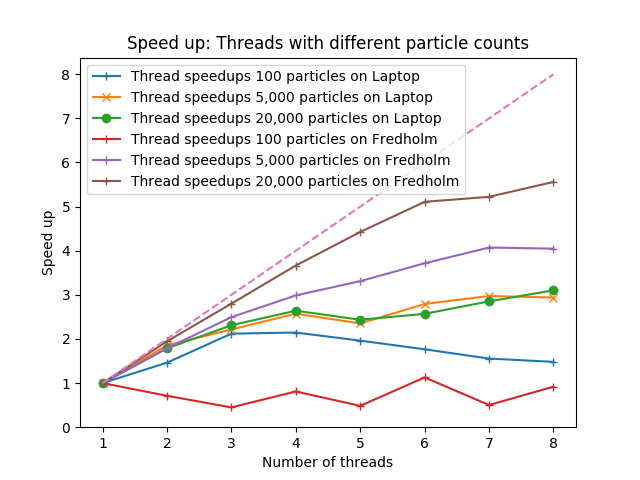
\includegraphics[width = 12cm]{../images/compute_pthreads.png}
    \caption{Speed up graphic: Pthread}
  \end{center}
\end{figure}
From the above graph, we can see that a smaller number of particles isn't affected too greatly with increased number of threads. The code seems to run slightly more efficiently on the laptop than the systems at university for the case of 100 particles.

The efficiency of the threads for the 5,000 and 20,000 particle systems on the laptop are fairly similar suggesting there is a peak speed up for file size with this number of threads.

However, if we keep increasing the file size on the Fredholm system, we get slightly better speed up results. A potential reason for not having an almost linear increase in performance through number of threads is due to the code not being completely parallelized. For instance, we did not parallelize the code for building the quadtree since, computationally, it took up a significantly smaller portion of time compared with that of the force computations.
